\documentclass[xcolor=dvipsnames]{beamer} % dvipsnames gives more built-in colors
\mode<presentation>

\usetheme{Boadilla}

\definecolor{GWdarkblue}{HTML}{033C5A}

\usecolortheme[named=GWdarkblue]{structure}

% Sets the font
\usepackage[defaultfam,tabular,lining]{montserrat}
\setbeamerfont{title}{shape=\scshape}
\setbeamerfont{frametitle}{shape=\scshape}
%Remove "Figure" from captions
\setbeamertemplate{caption}{\raggedright\insertcaption\par}

\usepackage{graphicx}
\usepackage{tabularx}
\usepackage{hyperref}

\title[Correlation vs. Causation]{Correlation vs. Causation}
\author[SMPA 2152]{Data Analysis for Journalism and Political Communication (Spring 2024)}
\date{Prof. Bell}

\begin{document}


%%%%%%%%%%%%%%%%%%%%%%%%%%%%%%%%%%%%%%%%%%%%%%%%%%%%%%%%%%%%%%%%%%
\frame{
\titlepage
}

%%%%%%%%%%%%%%%%%%%%%%%%%%%%%%%%%%%%%%%%%%%%%%%%%%%%%%%%%%%%%%%%%%
\frame{
\centering
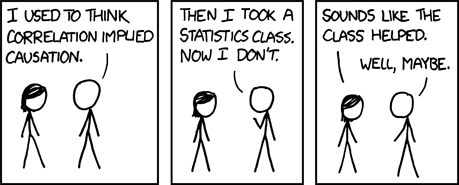
\includegraphics[width = .9\textwidth]{xkcd_correlation.png}
}

%%%%%%%%%%%%%%%%%%%%%%%%%%%%%%%%%%%%%%%%%%%%%%%%%%%%%%%%%%%%%%%%%%
\frame{
\only<1-2,4>{
    \begin{block}{Correlation}
    Correlation exists when the absolute rate of change in the values of two variables are similar.
    \end{block}
    ~\\
    \begin{itemize}
        \item<2-> \textbf{Positive correlation}: As the value of one variable increases (decreases), the value of the other variable increases (decreases) at the same rate
        \item<4-> \textbf{Negative correlation}: As the value of one variable increases (decreases), the value of the other variable decreases (increases) at the same rate
    \end{itemize}
}
\only<3>{
    \centering
    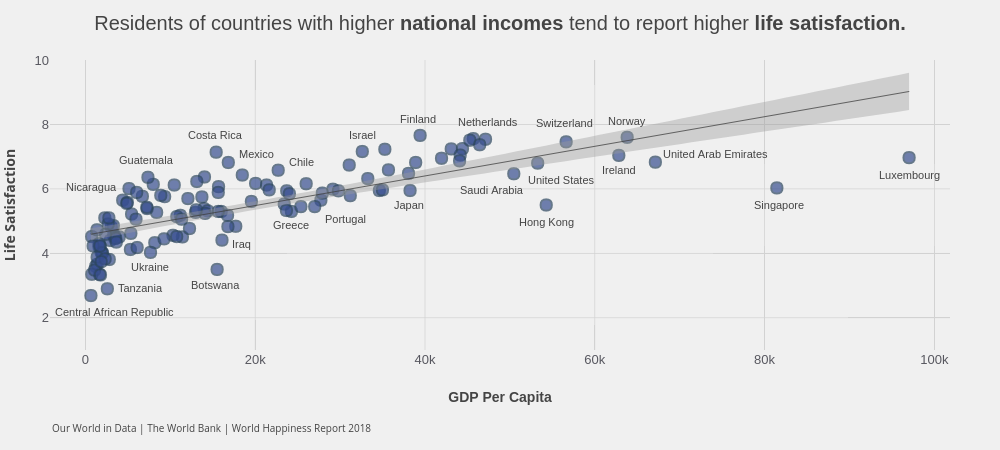
\includegraphics[width=.9\textwidth]{pos_correlation.png}
}
\only<5>{
    \centering
    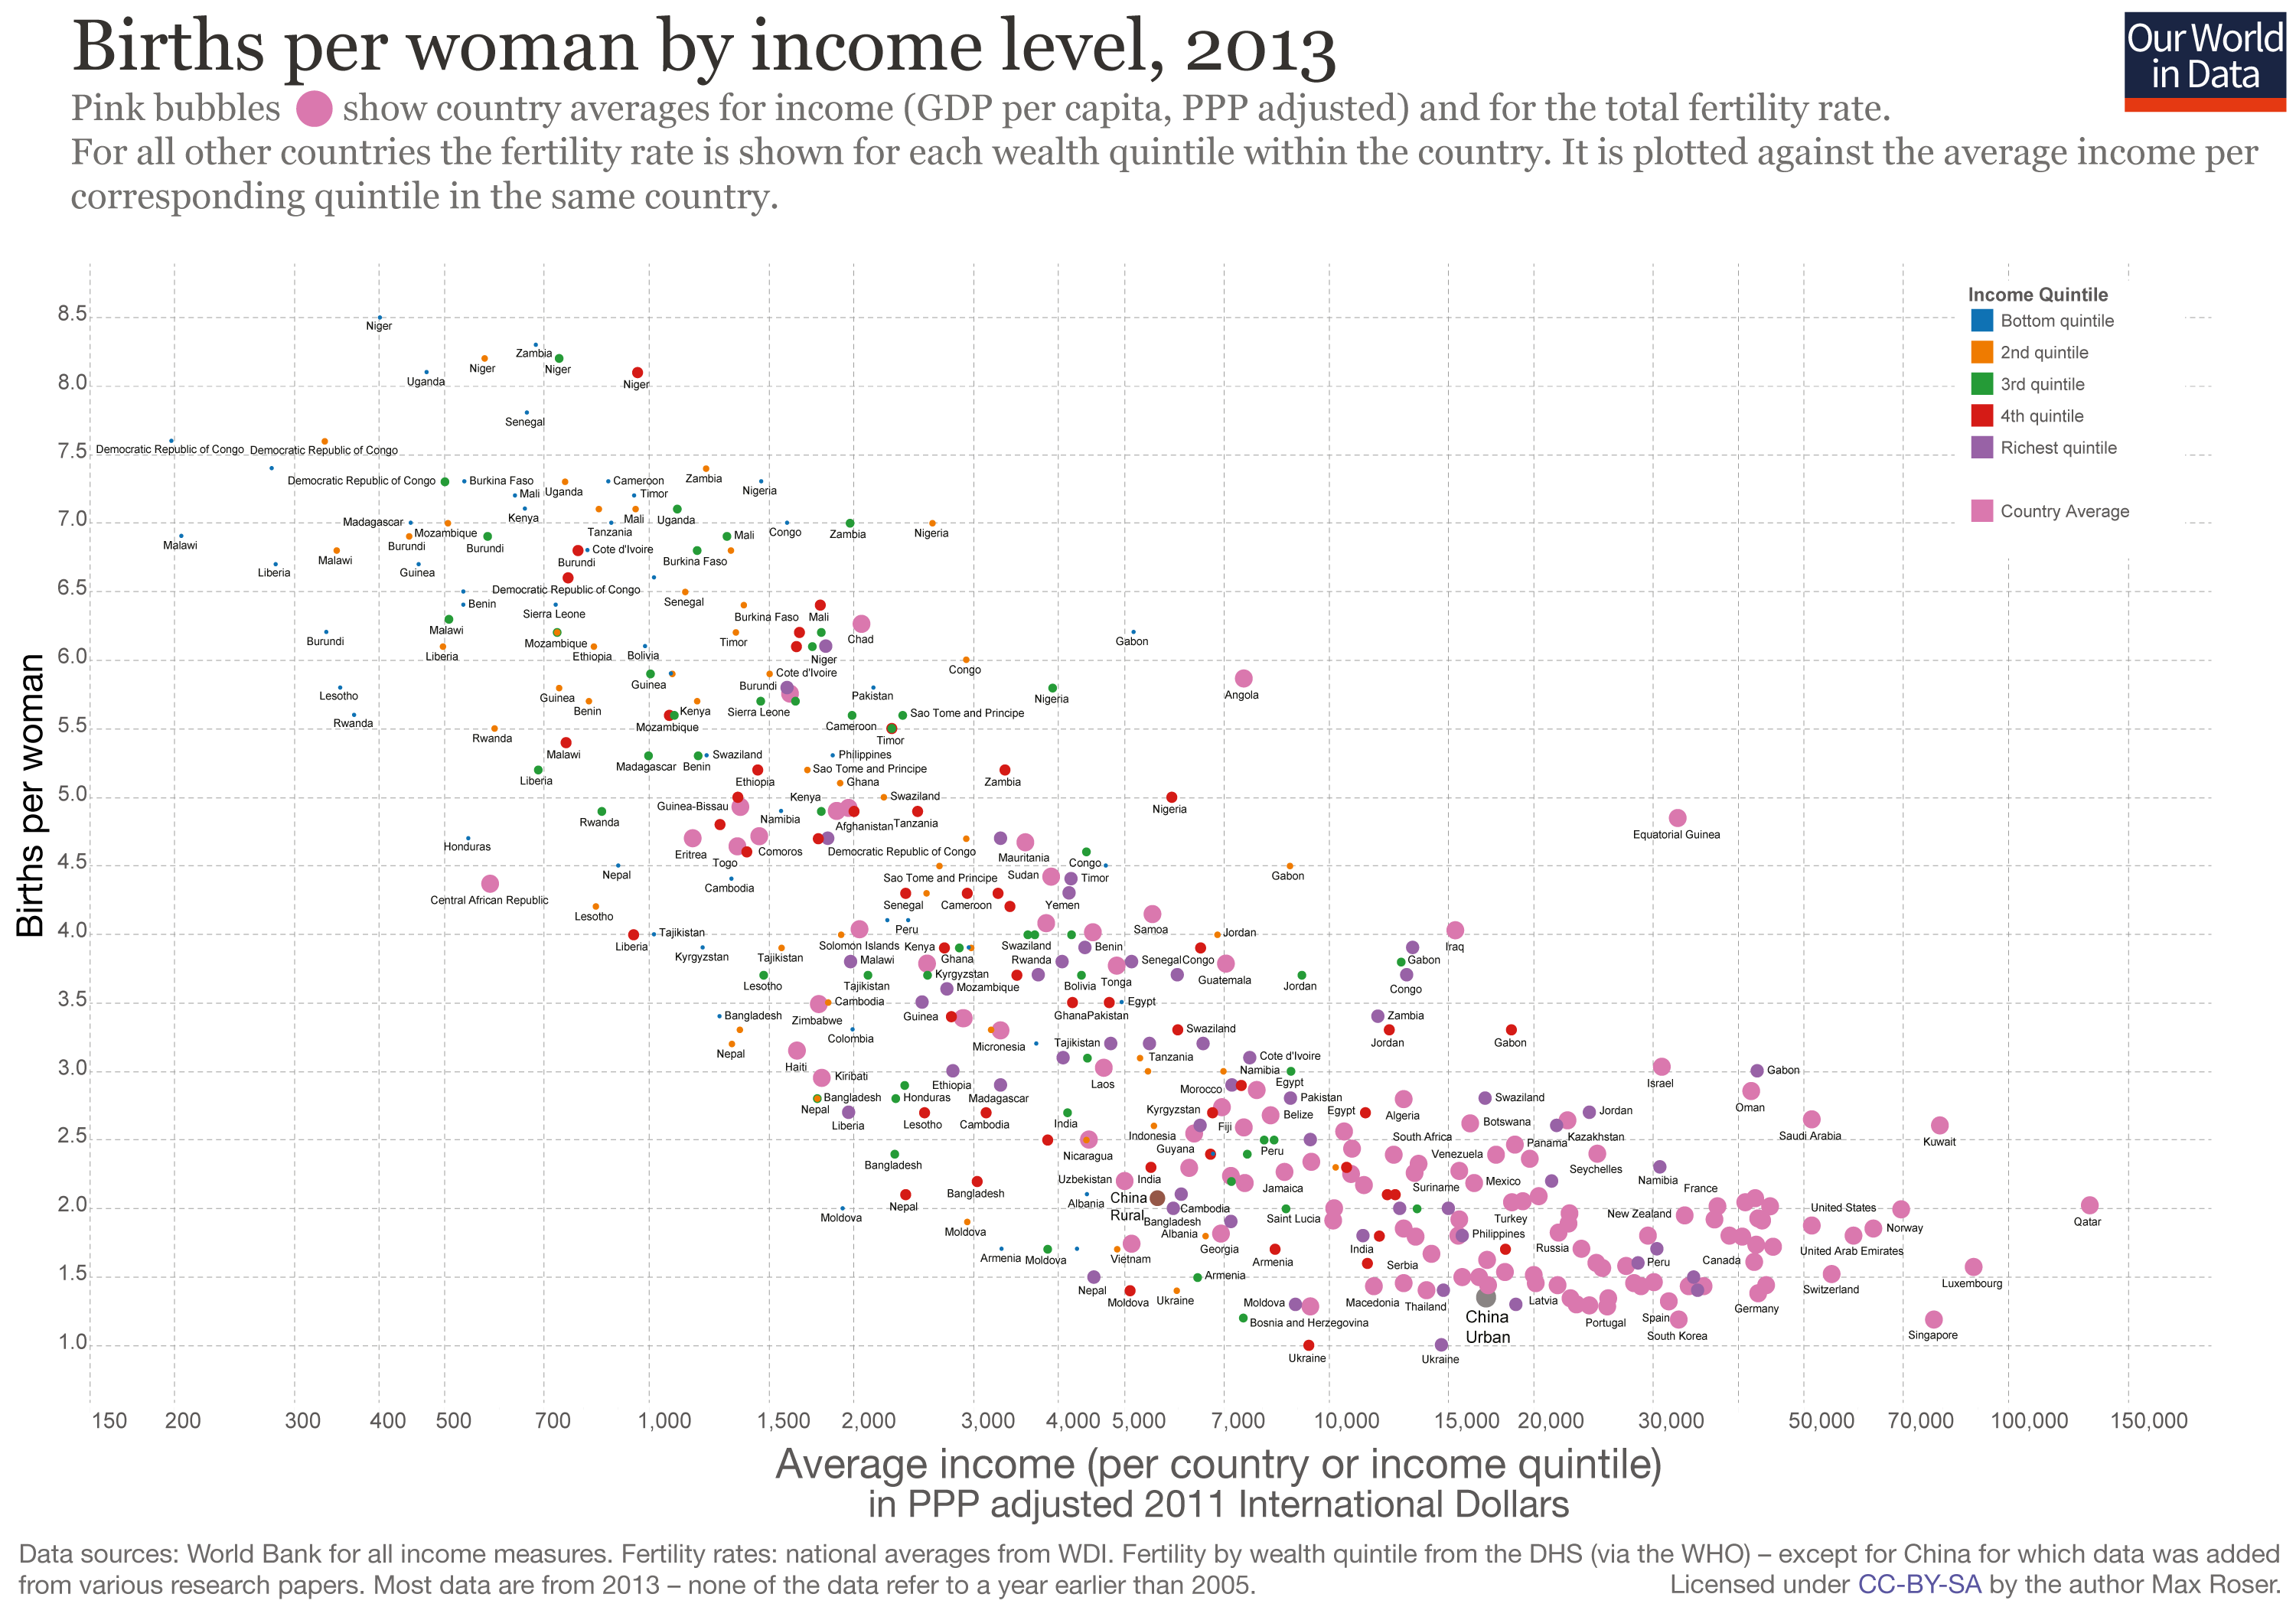
\includegraphics[width=.9\textwidth]{neg_correlation.png}
}
}

%%%%%%%%%%%%%%%%%%%%%%%%%%%%%%%%%%%%%%%%%%%%%%%%%%%%%%%%%%%%%%%%%%
\frame{
\only<1-4>{
    \begin{block}{Causation}
    Causation exists when a change in the value of one variable would not be observed without a preceding change in the value of another variable.
    \end{block}
    ~\\
    \begin{itemize}[<+(1)->]
        \item Correlation is descriptive, while causation is predictive
        \item We say that the \textbf{independent} or \textbf{explanatory} variable causes the \textbf{dependent} or \textbf{outcome} variable
        \item Causation depends on knowing the \textbf{counterfactual}: if we did not observe a change in the value of the explanatory variable, we would not observe a change in the value of the outcome variable
    \end{itemize}
}

\only<5>{
    \centering
    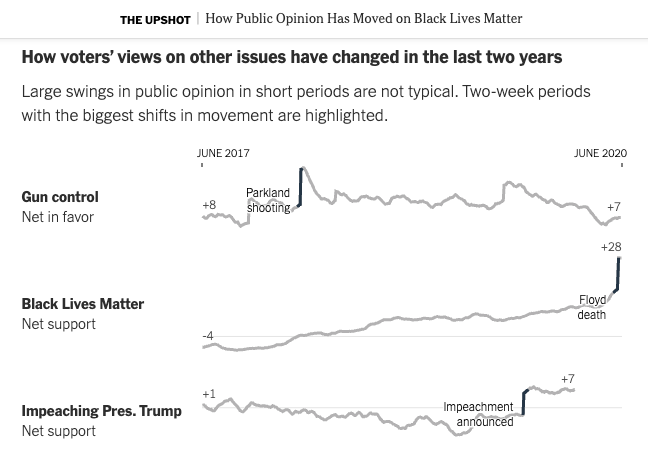
\includegraphics[width=.8\textwidth]{nyt_public_opinion.png}
}
\only<6>{
    \centering
    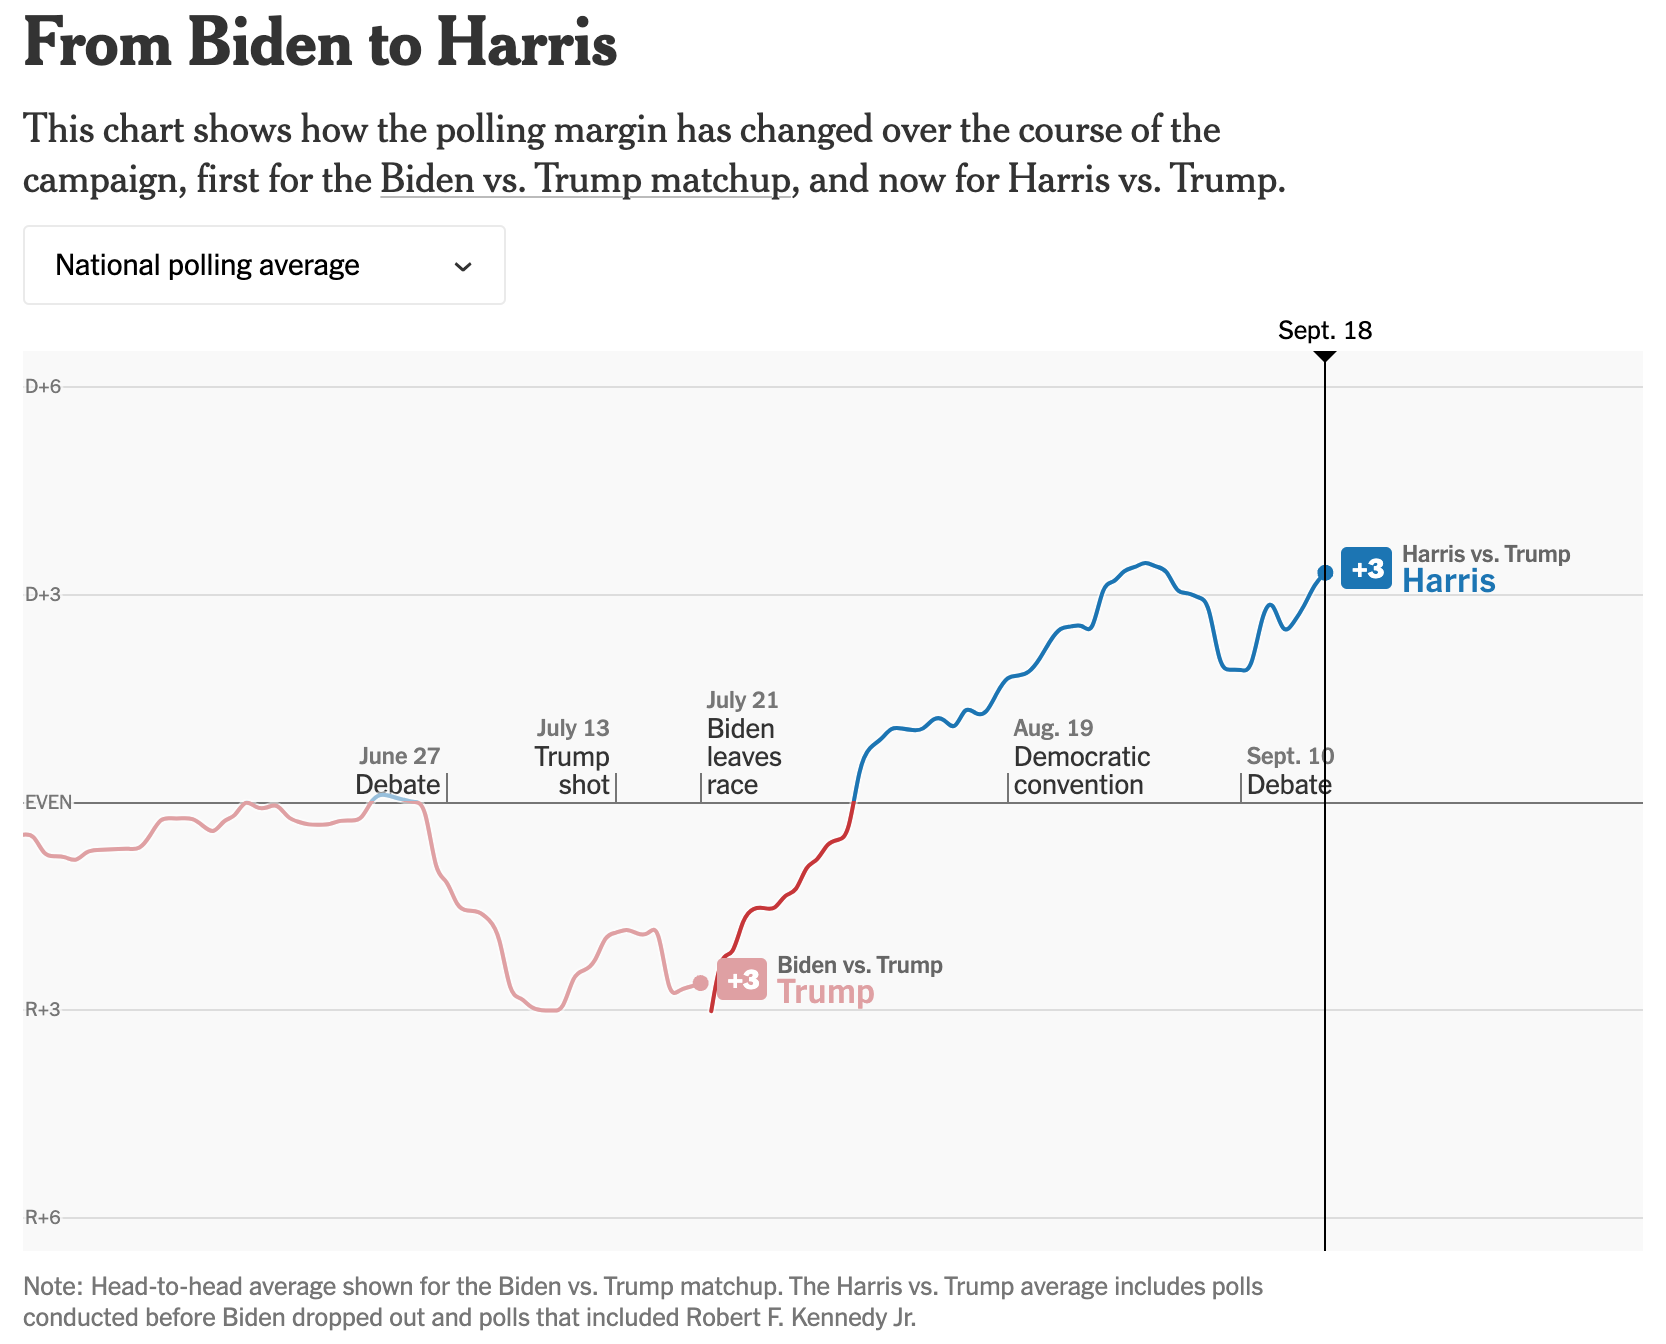
\includegraphics[width=.8\textwidth]{2024polls.png}
}
\only<7>{
    \centering
    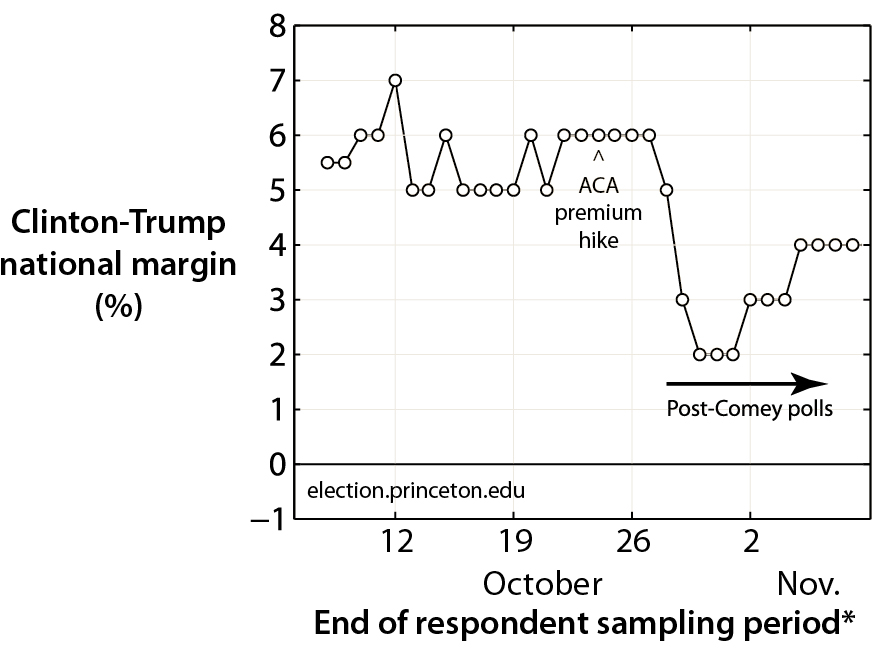
\includegraphics[width=.8\textwidth]{comey_letter.jpg}
}
}

%%%%%%%%%%%%%%%%%%%%%%%%%%%%%%%%%%%%%%%%%%%%%%%%%%%%%%%%%%%%%%%%%%
\frame{
\begin{block}{The Fundamental Problem of Causal Inference}
For any given case, we observe the outcome variable with \textit{either} a change in the independent variable or no change in the independent variable, but not both.
\end{block}
~\\
\begin{itemize}[<+(1)->]
    \item In other words, we do not observe the counterfactual
    \item But we try out best to observe the counterfactual using \textbf{experiments}
    \item Experiments establish a counterfactual by comparing cases that differ only in the explanatory variable that we are interested in
\end{itemize}
}

%%%%%%%%%%%%%%%%%%%%%%%%%%%%%%%%%%%%%%%%%%%%%%%%%%%%%%%%%%%%%%%%%%
\frame{
\only<1>{
\centering
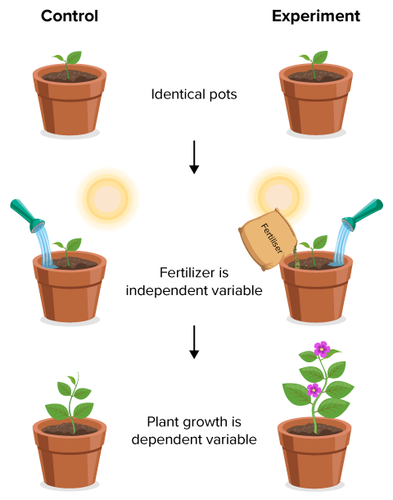
\includegraphics[height=.9\textheight]{plant_experiment.png}
}

\only<2>{\frametitle{John Snow's Cholera Experiment}
\centering
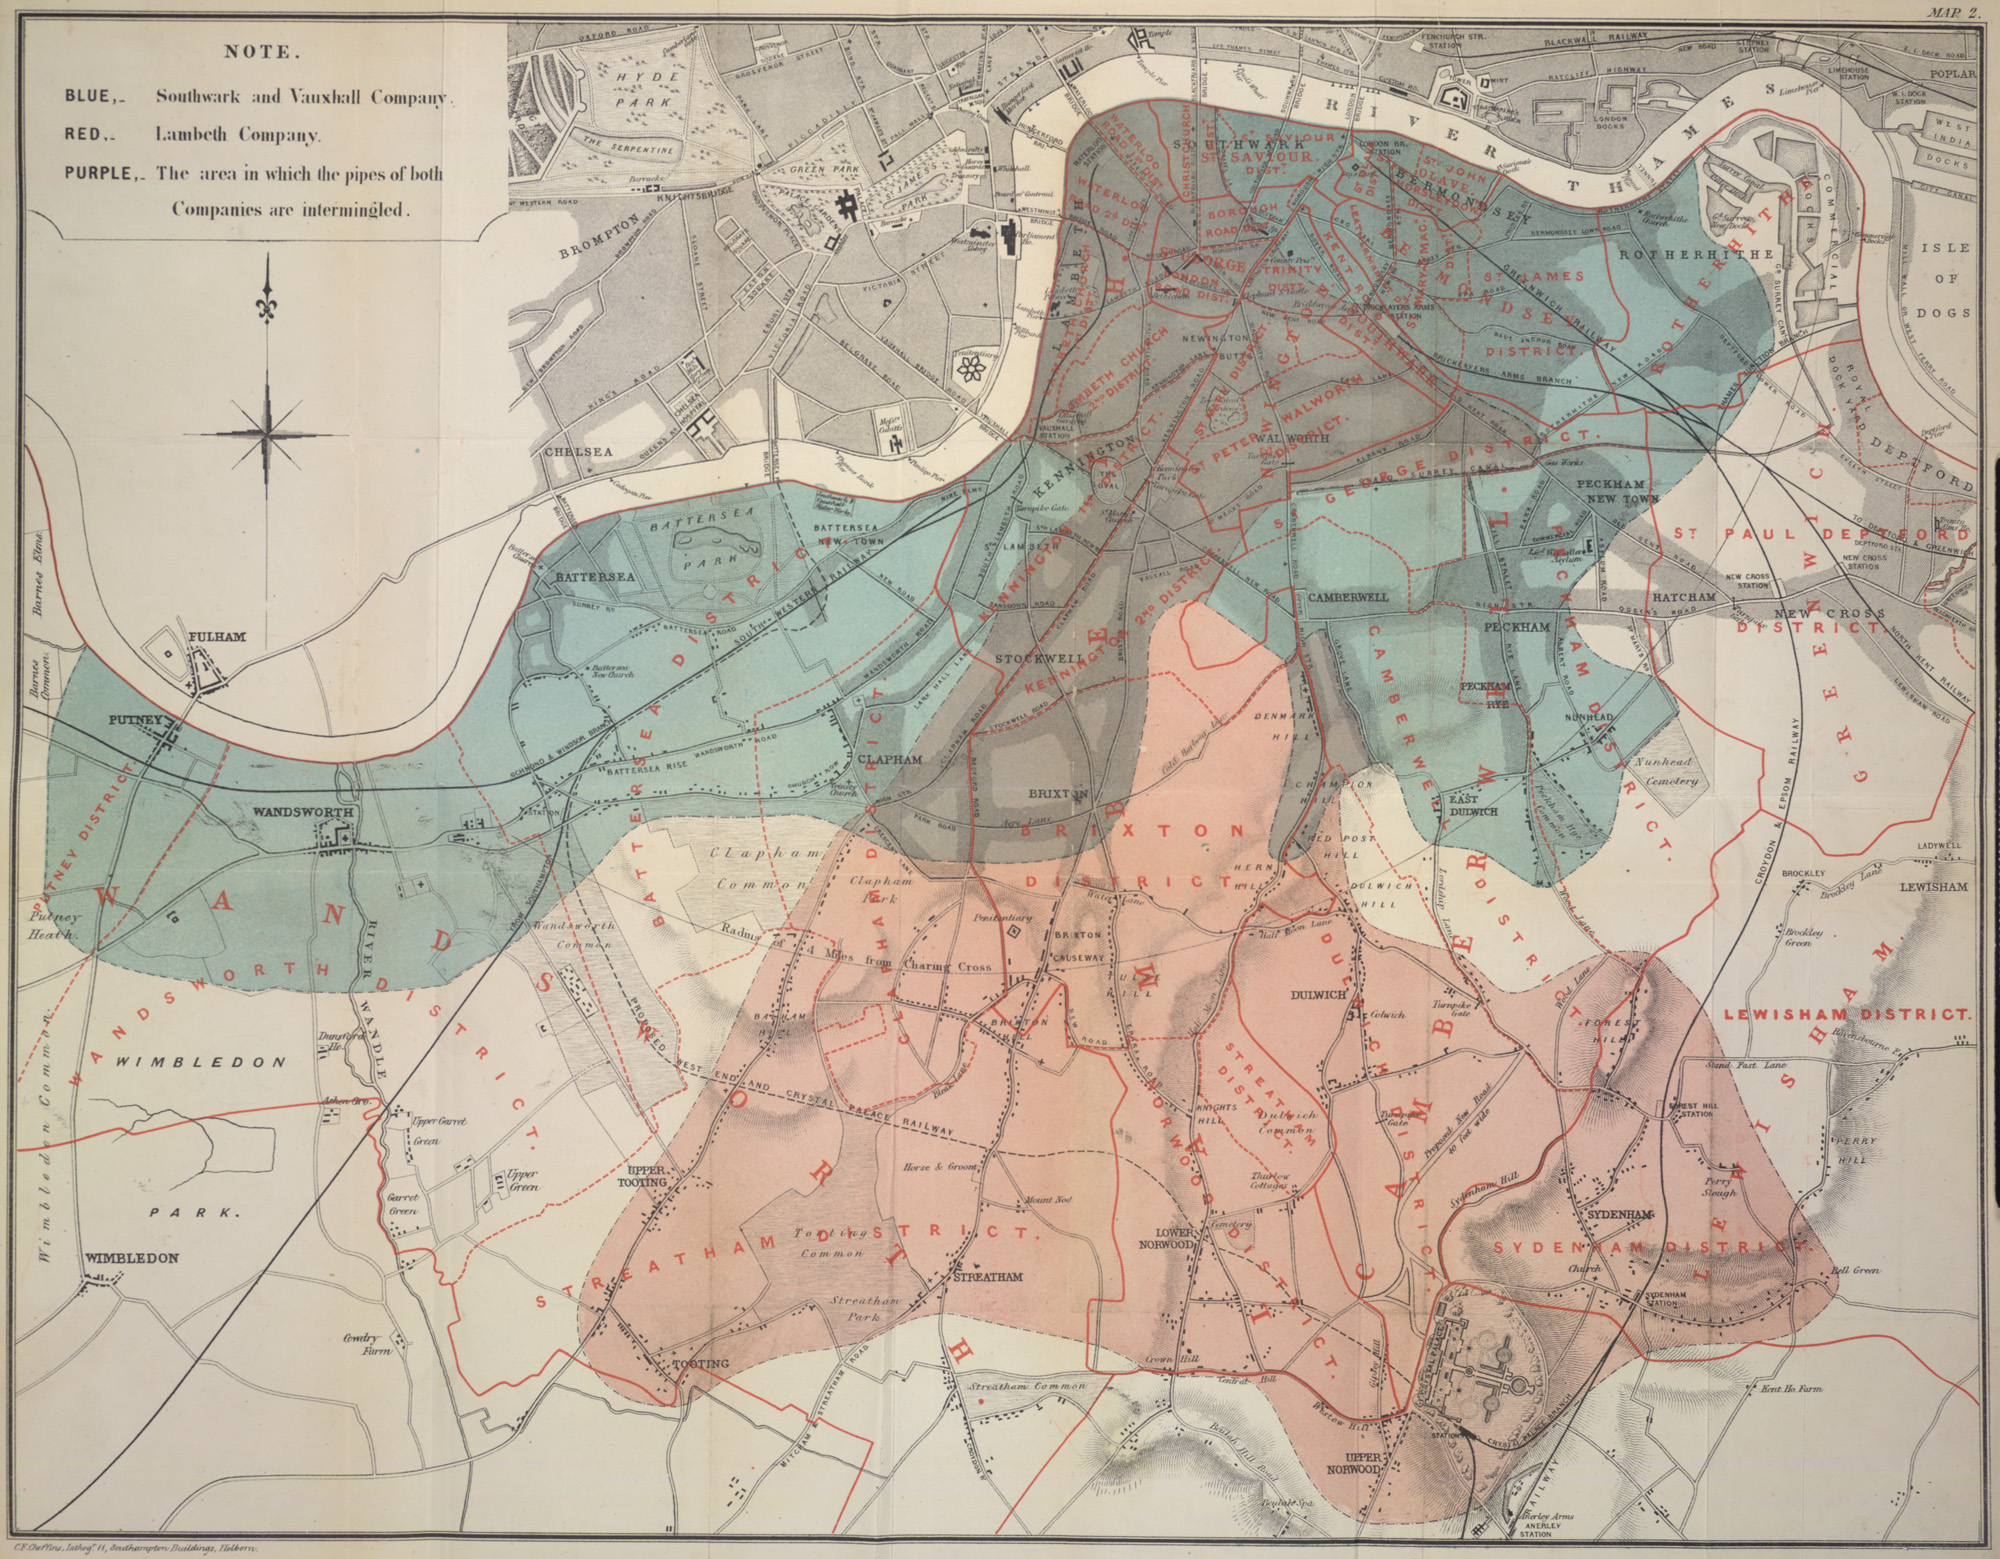
\includegraphics[width=.8\textwidth]{snow_map.jpg}
}

\only<3>{\frametitle{John Snow's Cholera Experiment}
\centering
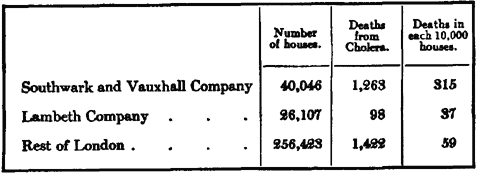
\includegraphics[width=.8\textwidth]{snow_results.png}
}
}

%%%%%%%%%%%%%%%%%%%%%%%%%%%%%%%%%%%%%%%%%%%%%%%%%%%%%%%%%%%%%%%%%%
\frame{\frametitle{Experiments}

\only<1-3>{
\begin{itemize}[<+->]
    \item A critical element of experiments is that the cases are assigned to the \textbf{treatment} group (e.g., getting a drug) and \textbf{control} group (e.g., getting a placebo) completely at random
    \item Recall the definition of a \textbf{random sample}: the probability of any given unit being drawn from the population is uniform (the same)
    \item The intuition for randomness is that there is no \textbf{selection bias}: patients aren't getting the drug because they are younger or healthier, for example.
\end{itemize}
}
\only<4-5, 7-8>{
\begin{itemize}[<+(3)->]
    \item But wait: were households in London assigned to either the Southwark \& Vauxhall Company or the Lambeth Company completely at random?
    \item No. This is called a natural experiment, and it relies on whether we believe being in either group is as-good-as-random.
    \item<7-> Finding natural experiments in the real world is really difficult, so we often design our experiments in controlled settings like laboratories or surveys
    \item<8-> We only have a true experiment where the \underline{researcher} randomly assigns cases to treatment or control.
\end{itemize}
}

\only<6>{
\centering
Card and Krueger (1994)\\
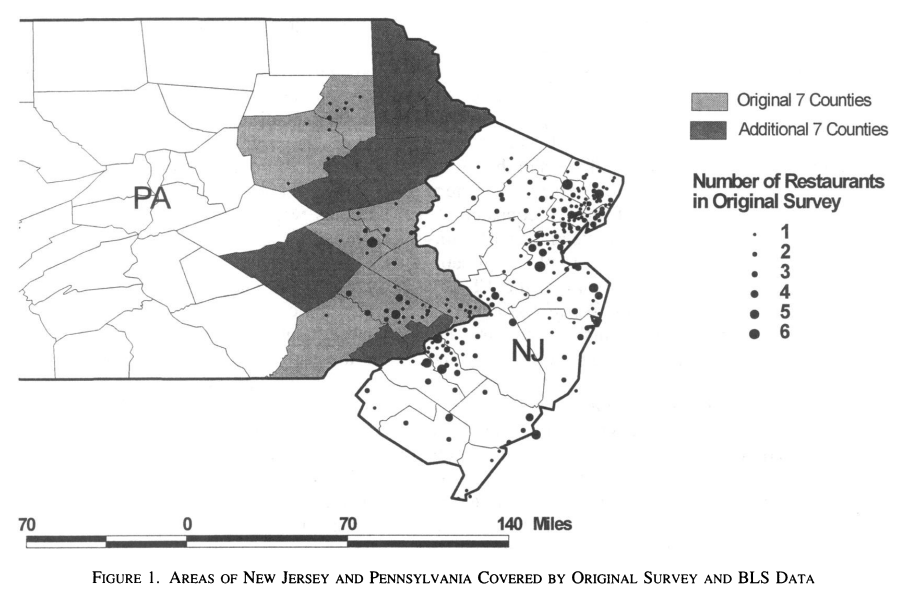
\includegraphics[width=.9\textwidth]{card_krueger.png}
}

\only<9>{
\centering
Kam and Zechmeister (2013)\\
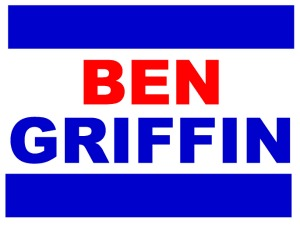
\includegraphics[width=.6\textwidth]{kam-zechmeister.jpg}
}

}

%%%%%%%%%%%%%%%%%%%%%%%%%%%%%%%%%%%%%%%%%%%%%%%%%%%%%%%%%%%%%%%%%%
\frame{\frametitle{Assessing Causality Without Experiments}

\only<1-3>{
\begin{itemize}[<+->]
    \item What about when we don't have an experiment, but instead are collecting \textbf{observational data} from the world?
    \item Then we face the fundamental problem of causal inference. Correlation does not imply causation.
    \item But all hope is not lost - we just have to be much more careful before making causal claims.
\end{itemize}
}

\only<4,7-8,11>{
\begin{itemize}
    \item<4-> Consider possible \textbf{confounders}: other variables that could explain the change in both the explanatory variable and the outcome variable
    \item<7-> Stronger associations are less susceptible to confounding
    \item<8-> Consider possible \textbf{reverse causation}, especially where the explanatory variable does not clearly precede the outcome variable
    \item<11-> Is there a plausible theory for how the explanatory variable causes the outcome variable?
\end{itemize}
}

\only<5>{
    \centering
    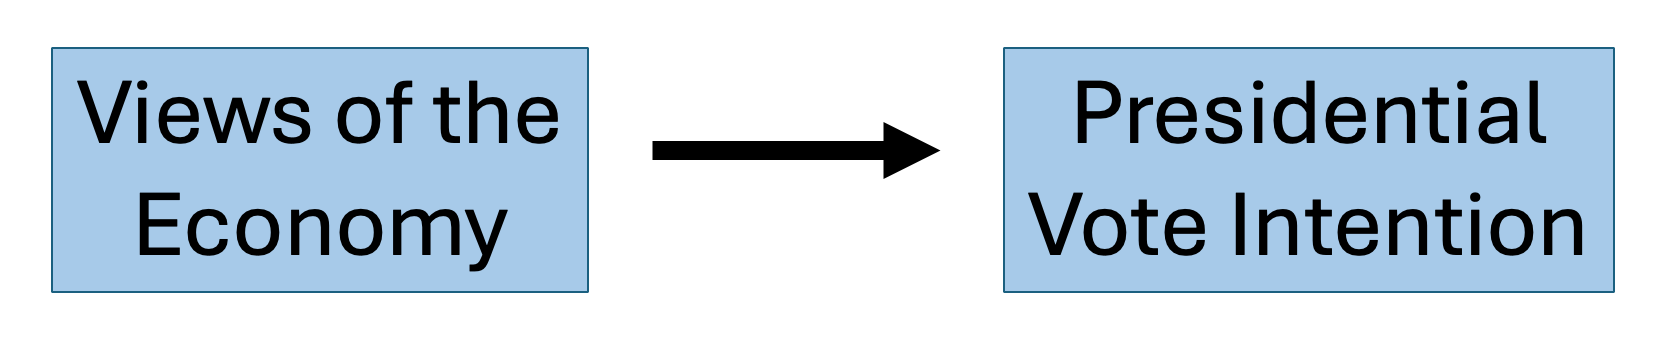
\includegraphics[width=.9\textwidth]{causal_diagram.png}
}
\only<6>{
    \centering
    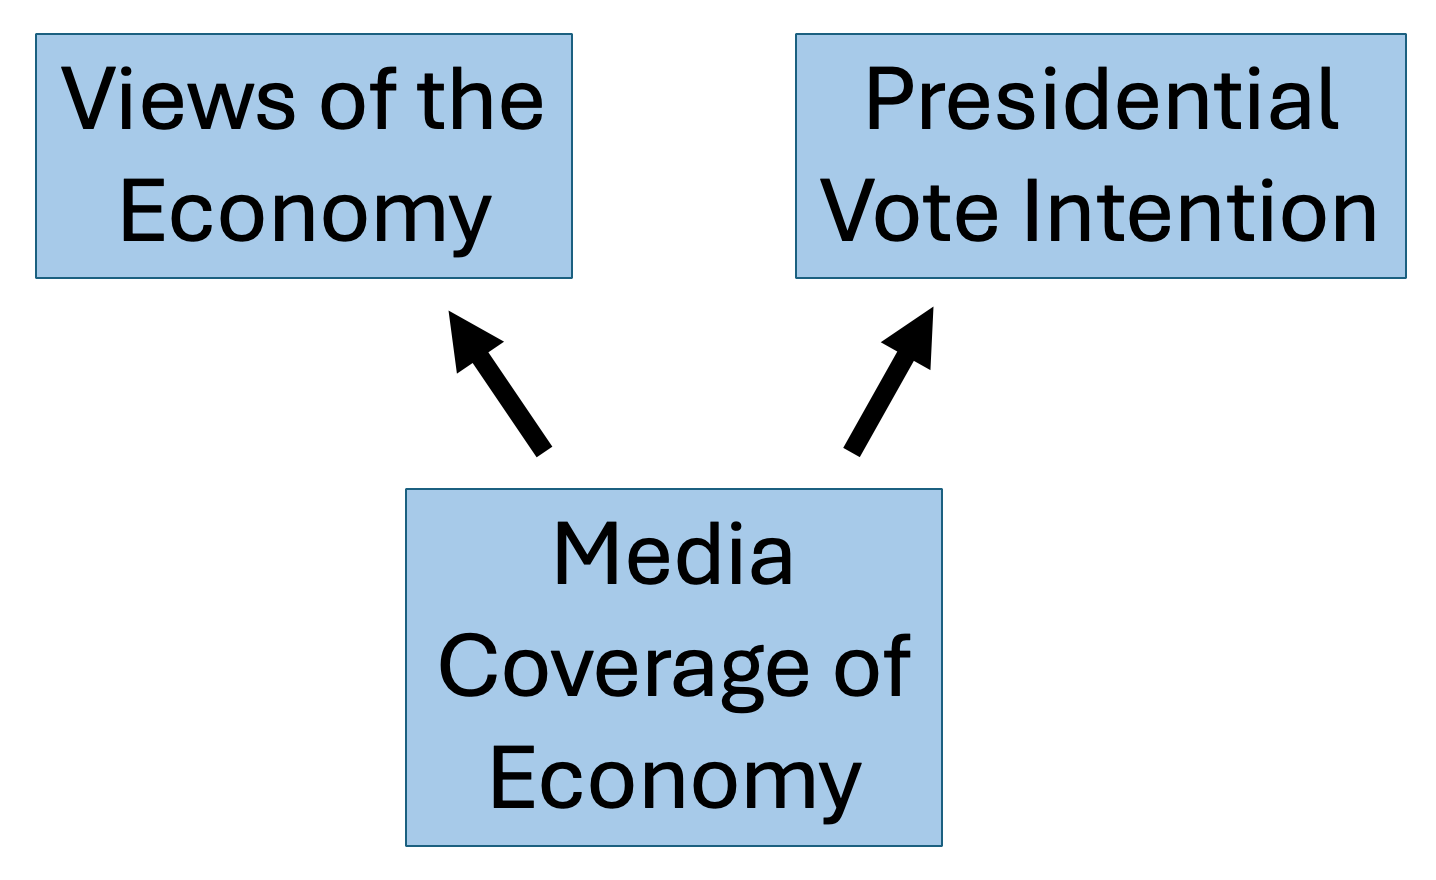
\includegraphics[width=.9\textwidth]{confounding.png}
}
\only<9>{
    \centering
    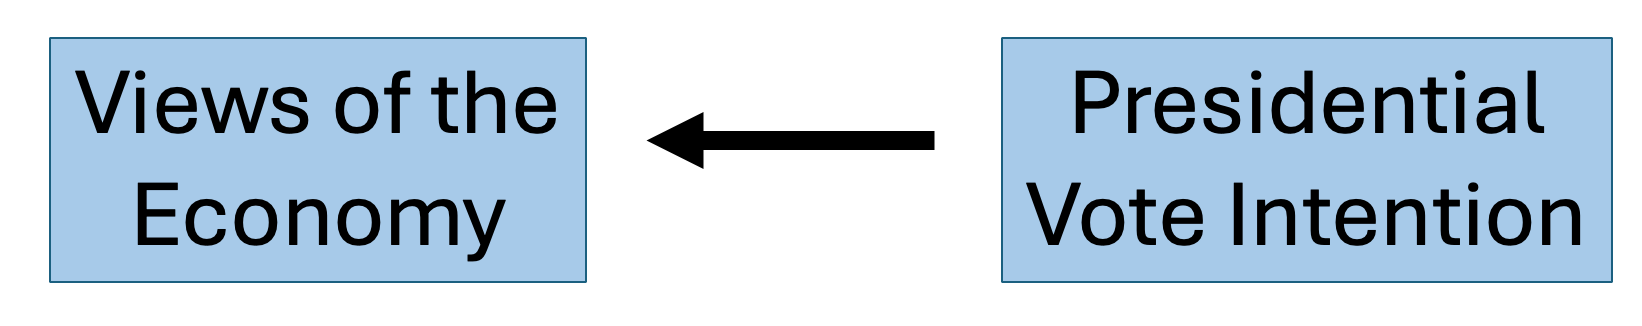
\includegraphics[width=.9\textwidth]{reverse_causation.png}
}
\only<10>{
    \centering
    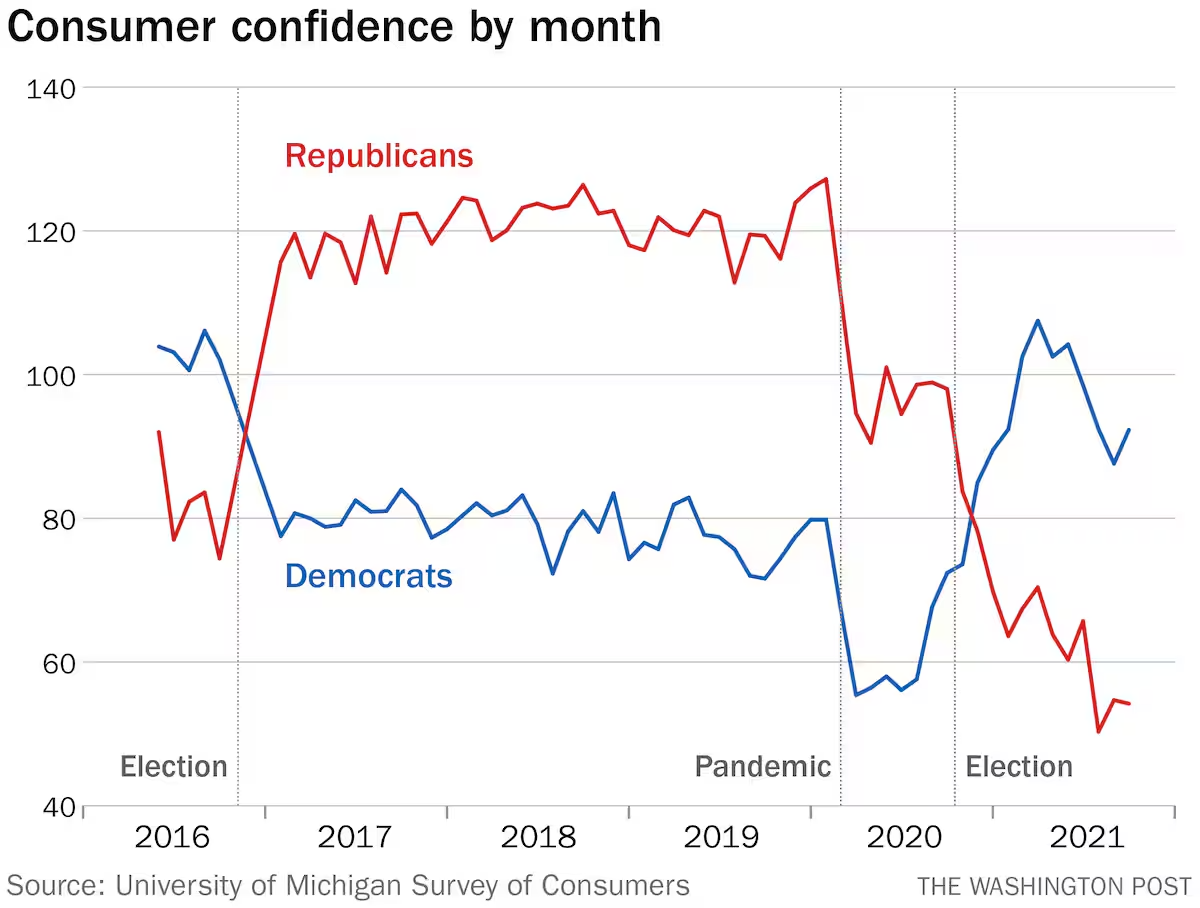
\includegraphics[width=.8\textwidth]{consumer_sentiment.png}
}
}

%%%%%%%%%%%%%%%%%%%%%%%%%%%%%%%%%%%%%%%%%%%%%%%%%%%%%%%%%%%%%%%%%%
\frame{
\centering
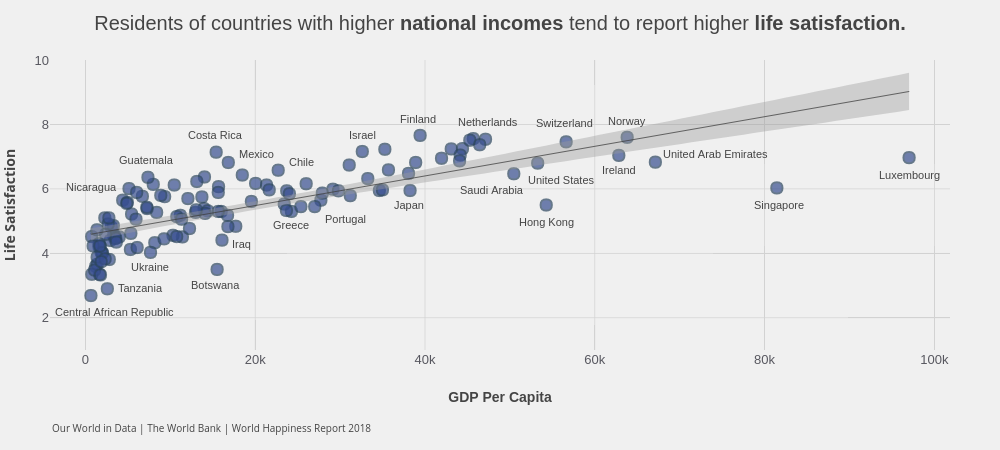
\includegraphics[width=.75\textwidth]{pos_correlation.png}\\
\begin{itemize}[<+->]
    \item The correlation between GDP per capita and life satisfaction could be stronger, so check for confounders
    \item Possible confounder: technological advancement increases economic productivity and provides entertainment
    \item Not clear that GDP per capita precedes happiness, so check for reverse causality
    \item Do happy people work harder?
\end{itemize}
}

%%%%%%%%%%%%%%%%%%%%%%%%%%%%%%%%%%%%%%%%%%%%%%%%%%%%%%%%%%%%%%%%%%
\frame{\frametitle{Exercise: Correlation vs. Causation}
}

%%%%%%%%%%%%%%%%%%%%%%%%%%%%%%%%%%%%%%%%%%%%%%%%%%%%%%%%%%%%%%%%%%
\frame{\frametitle{Conclusion}
\begin{itemize}
    \item Causation depends on knowing a counterfactual that we cannot observe (the fundamental problem of causal inference)
    \item Experiments overcome this issue by comparing groups that differ \underline{only} in their assignment to treatment or control (an artificial counterfactual)
    \item It is harder to make causal claims from observational data due to confounding and reverse causality
\end{itemize}
}

%%%%%%%%%%%%%%%%%%%%%%%%%%%%%%%%%%%%%%%%%%%%%%%%%%%%%%%%%%%%%%%%%%
\frame{\frametitle{"Conviction" by Rachel Aviv (New Yorker)}
\centering
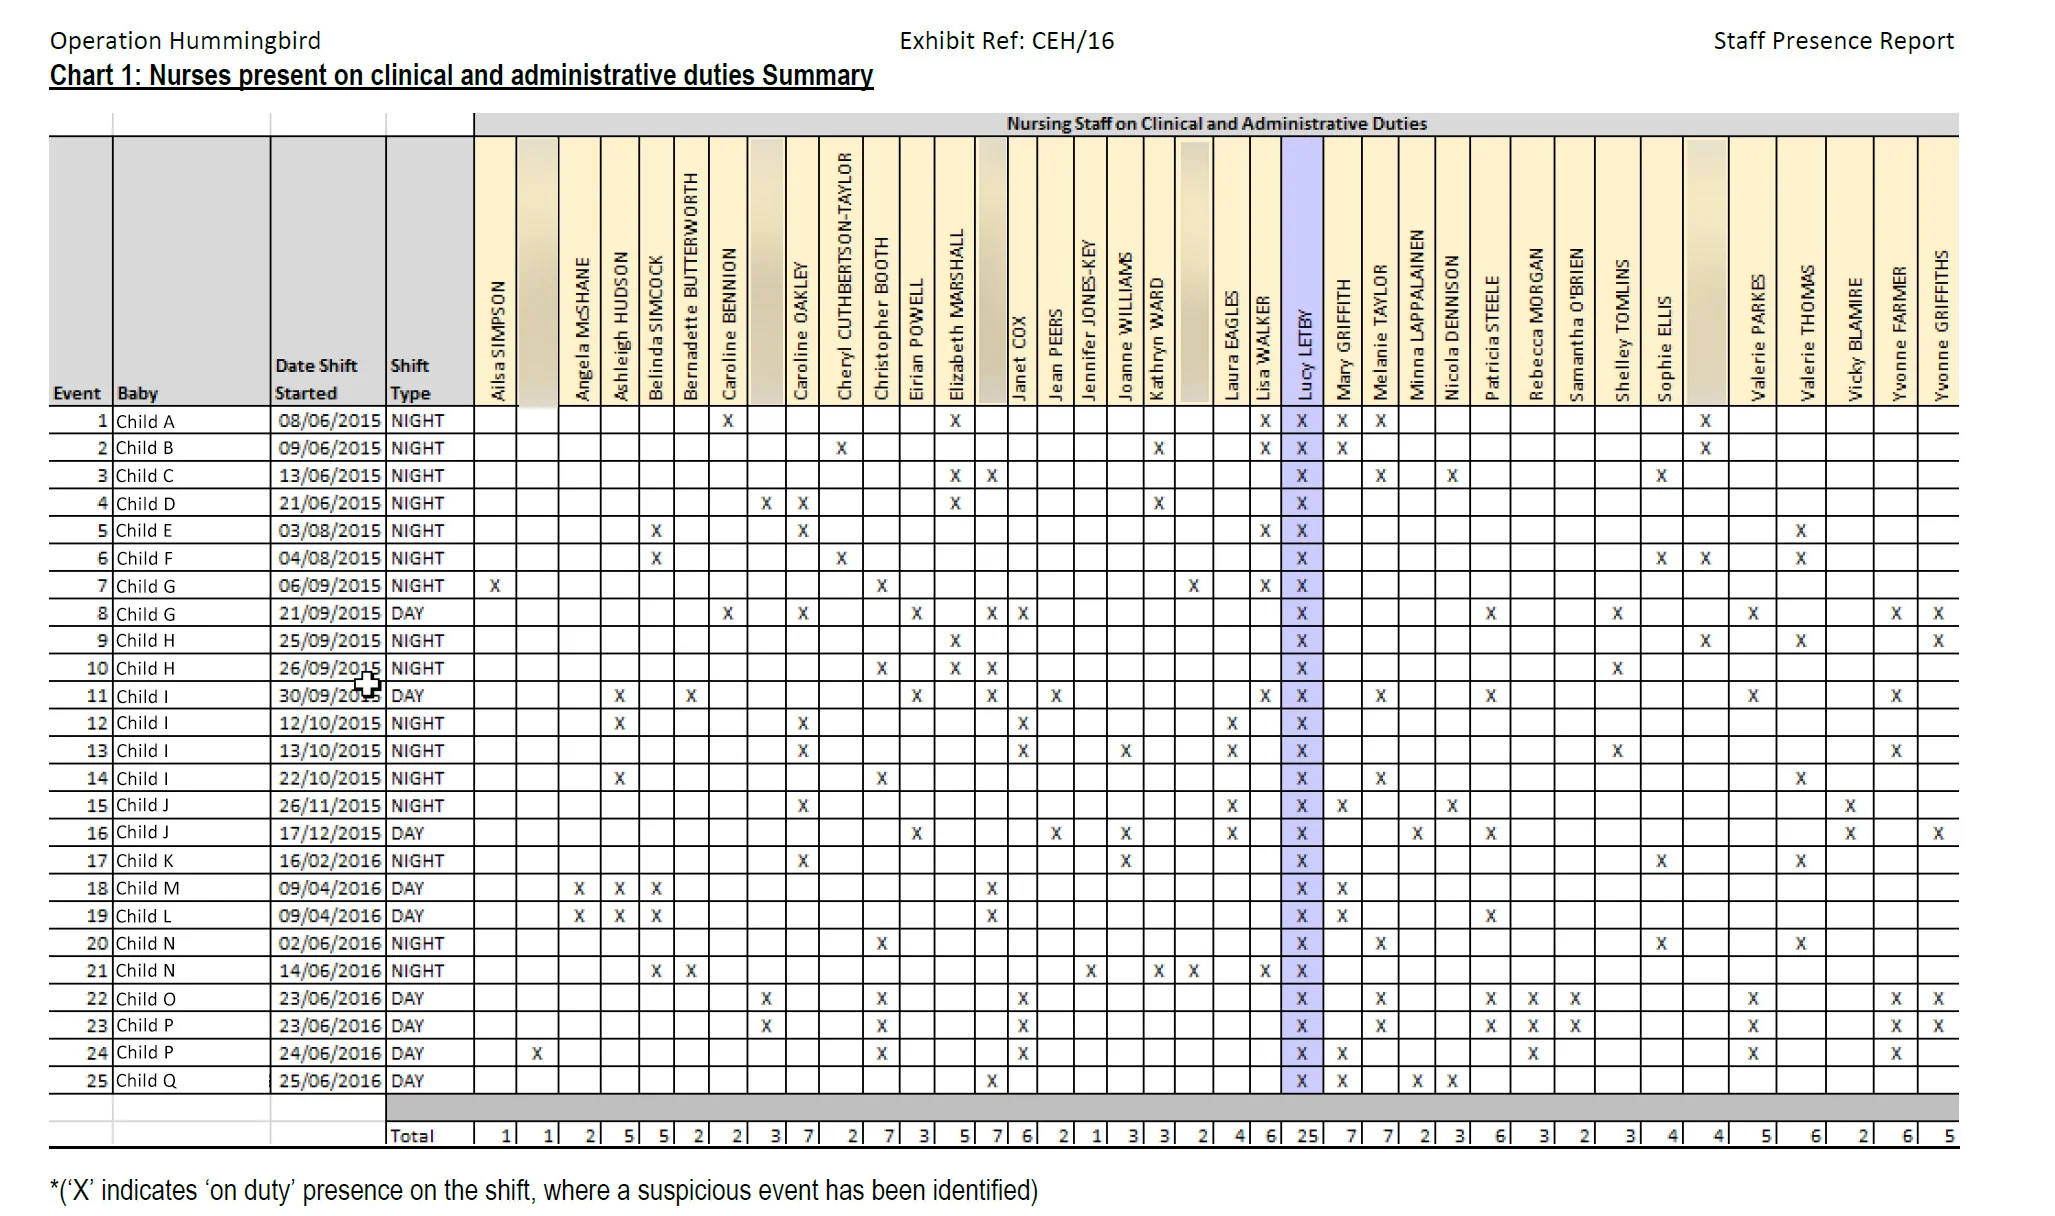
\includegraphics[width=\textwidth]{letby.png}
}

\end{document}
